\documentclass[
  version=last,
% Paper format
  paper=A4,
% Fontsize is 13pt, thus differing from BMCs version slightly.
% However this is necessary due to the Latex serif font being slightly smaller
  fontsize=13pt,
% Generate a seperate titlepage
  titlepage=true,
% Disables a seperating line between header and content
  headsepline=false,
% Enables a seperating line between footer and content
  footsepline=on,
% Use small headings with small spacings above and below
  headings=small,
% Bibliography is to be listed in the Table of Contents
  bibliography=totoc,
% The List of Tables and List of Figures are listed in the ToC
  listof=totoc
]{scrreprt}
% Set input encoding to UTF8... another possibility is utf8x, change if necessary 
\usepackage[utf8]{inputenc}
% Allows for special characters
% Since our font does not offer most of the symbols allowed by textcomp, we enable warn to display only warnings
% instead of errors, when font choice falls back to standard font (for the specific symbol only)
\usepackage[warn]{textcomp}
\usepackage{scrhack}
% Includes additional floats, see floats.tex
%Make own floats
\usepackage{float}
\makeatletter
%This changes the bmc float style to use the font settings as provided by (and set in) KOMAscript
%\newcommand\floatc@bmc[2]{\setbox\@tempboxa\hbox{{\@fs@cfont #1:} #2}%
%\ifdim\wd\@tempboxa>\hsize {\@fs@cfont #1:} #2\par
%\else\hbox to\hsize{\hfil\box\@tempboxa\hfil}\fi}
%\newcommand\fs@bmc{\def\@fs@cfont{\usekomafont{caption}\usekomafont{captionlabel}}\let\@fs@capt\floatc@plain
%\def\@fs@pre{}\def\@fs@post{}%
%\def\@fs@mid{\vspace\abovecaptionskip\relax}%
%\let\@fs@iftopcapt\iffalse} % NOTE: Some editors (e.g. Kile) will wrongly highlight this as an open-ended comment

%\floatstyle{bmc}
\floatstyle{komabelow}
\newfloat{code}{h}{bmccode}
%TODO port to language codes

%\renewcommand{\@fs@captfont}{\usekomafont{caption}}
\newfloat{bmceq}{h}{bmceq}

%Possible: \listof{<type}{<title>}
% Babel enables automatic hyphenation, translates titles of ToC, the listof* and bibliography
\newcommand{\langisgerman}{
% Sets the language to german by enabling the german babel package
  \usepackage[german]{babel}
  \selectlanguage{german}
  \newcommand{\seite}{Seite}
  \floatname{code}{Quellcode}
  \floatname{bmceq}{Gleichung}
  \newcommand{\bmceqlist}{Gleichungsverzeichnis}
  \newcommand{\codelist}{Quellcodeverzeichnis}
}
\newcommand{\langisenglish}{
% Sets the language to english by enabling the english babel package
  \usepackage[english]{babel}
  \selectlanguage{english}
  \newcommand{\seite}{Page}
  \floatname{code}{Source code}
  \floatname{bmceq}{Equation}
  \newcommand{\bmceqlist}{Table of Equations}
  \newcommand{\codelist}{Table of Source codes}
}
% Initialize variables, that must exist
\newcommand{\titel}{}
\newcommand{\untertitel}{}
\newcommand{\arbeitsart}{}
\newcommand{\studiengang}{}
\newcommand{\vorname}{}
\newcommand{\nachname}{}
\newcommand{\matrikelnummer}{}
\newcommand{\ort}{Essen}
\newcommand{\datum}{\today}
\newcommand{\betreuer}{}
%%%%%%%%%%%%%%%%%%%%%%%%%%%%%%%%%%%%%%%%
% Include variables as set by the user
% This should overwrite all previously initialized variables
% Setze die Sprache deines Papers. Die nicht verwendete Sprache auskommentieren
%\langisgerman
\langisenglish
%%%%%%%%%%%%%%%%%%%%%%%%%%%%%%%%%%%%%%%%%%%%%%
% Setze den Titel deines Papers
\renewcommand{\titel}{Evaluation of a lightweight debugging platform for mobile sensor networks}
% Setze den Untertitel deines Papers
\renewcommand{\untertitel}{}
% Setze die Art der Arbeit
\renewcommand{\arbeitsart}{Bachelor}
% Setze die Bezeichnung deines Studienganges
\renewcommand{\studiengang}{Angewandte Informatik - Systems Engineering}
% Setze deinen Vornamen
\renewcommand{\vorname}{Michael}
% Setze deinen Nachnamen
\renewcommand{\nachname}{Krane}
% Setze deine Matrikelnummer
\renewcommand{\matrikelnummer}{2233018}
% Setze den Ort, an dem dein Paper verfasst wurde
% Das % hinter dem Ort nicht löschen!
\renewcommand{\ort}{Essen}
% Setze den Namen des Betreuers hier ein
\renewcommand{\betreuer}{Hugues Smeets}
%%%%%%%%%%%%% OPTIONALER TEIL %%%%%%%%%%%%%
% Setze den Namen deines Erstgutachters, andernfalls auskommentieren
\newcommand{\erstgutachter}{Prof. Dr. Pedro José Marrón}
% Setze den Namen deines Zweitgutachters, andernfalls auskommentieren
\newcommand{\zweitgutachter}{Prof. Dr. Gregor Schiele}
% Falls ein anderes Datum als das aktuelle verwendet werden soll, muss dies hier eingesetzt werden 
%\renewcommand{\datum}{%
%\today
%}
% Set title, date and name... this is not used, but KOMA script complains if they are not set
\title{\titel}
\date{\datum}
\newcommand{\firstname}{\vorname}
\newcommand{\lastname}{\nachname}
% Allows the use of images in the figure-environment
\usepackage{graphicx}
% head = 2cm includes header and headsep
\usepackage[
% Left margin as in BMCs version
  left=2.5cm,
% Right margin as in BMCs version
  right=2.5cm,
% The top differs slightly from BMCs version due to LaTeX including header and footer in the respective margins
  top=2.5cm,
% See top
  bottom=2.25cm,
% 28.3464567pt = headheight + headsep
% In case you did not know or just forgot: 1 inch = 72pt
% Height of the entire text body should be 25cm, equal 708.... pt
  textheight=708.661418pt,
% Footskip is the size of the footer
  footskip=0.95cm,
% Headheight should be just high enough for a single line
  headheight=8pt,
% The space between header and text body
  headsep=30pt,
]{geometry}
%\usepackage{layout} % Used for debugging purposes
% Used for linespacing
\usepackage{setspace}
% Include Helvetica als sans serif font
%\usepackage{helvet}              %<<<<<<<<<<<<<<<<<<<<<<<<<<<<<<<<<<<<<<<<<<<<<<<<<<<< UNCOMMENT TO CHANGE FONT
%\usepackage[T1]{fontenc}         %<<<<<<<<<<<<<<<<<<<<<<<<<<<<<<<<<<<<<<<<<<<<<<<<<<<< UNCOMMENT TO CHANGE FONT
% Include ifthenelse, used on the titlepage
\usepackage{ifthen}
% Allows referencing the last page, which is used to display the last page in the page counter
\usepackage{lastpage}
% The math, it hurts my brain!
\usepackage{amsmath}
\usepackage{amssymb}
% Here we create custom headers
\usepackage{scrpage2}
\pagestyle{scrheadings}
% Usually chapterpagestyle is scrplain, but we do not use scrplain
\renewcommand{\chapterpagestyle}{scrheadings}
\newcommand{\beginformalia}{
% Switch to Roman page numbering (e.g. I, II, III, IV,...) for anything up to and including the Table of Contents
  \pagenumbering{Roman}
% Switches to Roman chapter numbering, should not be used usually, just for archival purposes in here
%\renewcommand{\thechapter}{\Roman{chapter}}
% Clear header and footer
  \clearscrheadfoot
% Enable automatic updates of the headmark
  \automark[section]{section}
% Sets the line seperating footer from text
  \setfootsepline{1pt}
% Sets the Roman page numbering during the preamble on the right bottom
  \ofoot[\pagemark]{\pagemark}
% Sets the paper title on the left bottom
  \ifoot[\titel]{\titel}
% Sets the left top to the current section number and title
  \ihead[\headmark]{\headmark}
}
\newcommand{\begincontent}{
% Switch to usual page numbering
  \pagenumbering{arabic}
% Resets chapter counter
  \setcounter{chapter}{0}
% Switches to arabic chapter numbering
  \renewcommand{\thechapter}{\arabic{chapter}}
% Changes the page numbering scheme 
  \ofoot[{\seite} {\pagemark}/\pageref{LastPage}]{{\seite} {\pagemark}/\pageref{LastPage}}
}
% Sets the numbering scheme of figures and tables to ignore the chapter number
% Usually it would be like "Figure 3.1: Some picture" in chapter 3
\usepackage{chngcntr}
\counterwithout{figure}{chapter} 
\counterwithout{table}{chapter}
% Allows citation
\usepackage{cite}
% Use the IEEE bibliography style
\bibliographystyle{IEEEtran}
% Colored tables
%\usepackage{colortbl}
%\arrayrulecolor{black}
% Includes the tabularx environment, which automatically stretches to accomodate a certain width
\usepackage{tabularx}
% Includes the longtable environment, which allows for tables to span across multiple pages
\usepackage{longtable}
% Reduces the space skipped at the top of the page when a new chapter starts
\renewcommand{\chapterheadstartvskip}{\vspace*{-30pt}}
% Adds a 12 pt skip after a chapter
\renewcommand{\chapterheadendvskip}{\vspace*{12pt}}
% Change default font to serif font
\renewcommand{\familydefault}{\sfdefault}
% Skip 3pt after every paragraph (also used in BMCs version)
\parskip 3pt
% No paragraph indentation
\parindent 0pt
%%%%%%%%%%%%%%%%%%%%%%%%%%%%%%%%%%%%%%%%%%%%%%%%%%%%%%%%%%%%%%%%%%%%%%%%%%%%%%%%%
% Allows links inside the paper and sets a few settings for the pdf like a correct headline displayed in a PDF reader
% and so on
\usepackage[
  pdftitle={\titel},
  pdfauthor={\vorname \nachname},
  pdfsubject={\vorname \nachname: \titel},
  colorlinks=true,
  linkcolor=black,
  citecolor=black,
  urlcolor=black
]{hyperref}
% Enables spacing changes around headlines (not usable on \chapter because KOMA script uses its own version or
% something, hence the above changes in \chapterhead{start,end}vskip)
% Sets 6 pt spacing after headings
\usepackage[compact]{titlesec}
\titlespacing{\section}{0pt}{6pt}{*0}
\titlespacing{\subsection}{0pt}{6pt}{*0}
\titlespacing{\subsubsection}{0pt}{6pt}{*0}
% Set fontsizes according to BMCs version
% Note that these font sizes will scale with changes of 'fontsize' as set in the documentclass settings
\setkomafont{section}{\large\bfseries\sffamily}
\setkomafont{subsection}{\normalsize\bfseries\sffamily}
\setkomafont{subsubsection}{\normalsize\mdseries}
\setkomafont{paragraph}{\normalsize\mdseries}
\setkomafont{subparagraph}{\normalsize\mdseries}
\setkomafont{pageheadfoot}{\scriptsize}
\setkomafont{caption}{\small}
% Enlarge widow and club penalty (up to 10000)
% This prevents widows and clubs completely to match the original behaviour
\clubpenalty=10000
\widowpenalty=10000
\begin{document}
% Limits hyphenation at line endings to match the behaviour in BMCs version
\sloppy
%\layout % Debugging purposes, should be commented out
%%%%%%%%%%%%%%%%%%%%%%%%%%%%%%%%%%%%%%%%%%%%% FRONTMATTER
% Include title page
%Herausgeber: 
%Prof. Dr. B. Müller-Clostermann
%Institut für Informatik und Wirtschaftsinformatik, Universität Duisburg-Essen, Campus Essen
%www.icb.uni-due.de
%Stand: 22.12.2010
%
%Portierung von Word zu LaTeX von Markus Kempe für den Lehrstuhl Technik der Rechnernetze

\begin{titlepage}
\rule{\textwidth}{0.4pt} \\[48pt]
\begin{center}
\begin{spacing}{2}
\textbf{\textsf{\Huge \titel}} \\
\textsf{\Large \untertitel}\\[52pt]

\textsf{\Large {\arbeitsart}arbeit im Studiengang {\studiengang} am Institut für Informatik und
Wirtschaftsinformatik der Universität Duisburg-Essen}\\[36pt]
\textbf{\textsf{\Large {\vorname} {\nachname} \\ {\matrikelnummer}}}\\[26pt]
\textbf{\textsf{\Large {\ort}, \datum}}
\end{spacing}
\end{center}
\textbf{Betreuer: \betreuer \\
\ifx\erstgutachter\undefined
\else
Erstgutachter: \erstgutachter \\
  \ifx\zweitgutachter\undefined
  \else
  Zweitgutachter: \zweitgutachter \\
  \fi
\fi
}
\end{titlepage}
% Set header and footer, use roman chapter numbering and so on
\beginformalia
% Include several files
\addchap{Abstract}
	\textbf{TODO}

\addchap{Zusammenfassung}
	\textbf{TODO}

% Abbildungsverzeichnis
\listoffigures
 \newpage
% Tabellenverzeichnis
%\listoftables
% \newpage
% Gleichungsverzeichnis
%\listof{bmceq}{\bmceqlist}
% \newpage
% Quellcodeverzeichnis
\listof{code}{\codelist}
\newpage
% Inhaltsverzeichnis
\tableofcontents 
\newpage


% Change header and footer, use arabic numbering and so on
\begincontent
%%%%%%%%%%%%%%%%%%%%%%%%%%%%%%%%% INHALT %%%%%%%%%%%%%%%%%%%%%
%Comment out the following line and uncomment the one after that when you are ready to start
\chapter{Introduction}
\label{sec:intro}
\textbf{TODO}
\begin{itemize}
	\item{Explain Context in which SHAMPU was designed}
	\item{Explain Problem SHAMPU tries to fix}
	\item{Explain "Problem" of this thesis "ANT as an addition to SHAMPU, need to know how good ANT is"}
	\item{Explain how problem was solved, e.g. Different experiments which try to evaluate ANT in the context of SHAMPU}
\end{itemize}
In this thesis we evaluate the WSN testbed: SHAMPU (Single chip Host for Autonomous Mote Programming over USB). 


\section{Related work}
\label{sec:related_work}

There are already several different WSN testbeds available. These testbeds all fulfil certain roles, but ultimately fail to provide all the necessary features for a small, mobiles and low power WSN testbed.\\

There are some testbeds which need a fixed infrastructure, like FlockLab \cite{Lim2013} or Minverva \cite{Sommer}. The nature of a fixed infrastructure has certain problems. For once it might only be  viable to test inside the lab and not in the target environment since the needed infrastructure is often only available inside a lab or not easily transportable. 

Other technologies aim to detach the testbed from the infrastructure itself and rely on wireless communication instead. Sensei-UU \cite{Rensfelt2009} for example uses a wireless 802.11 network for communication between the nodes and the sensor host. The problem here is the power requirements for the communication, which makes it hard to run the nodes without an external power source.

BTNodes \cite{Moser} or Smart-Its \cite{Kasten2000} use Bluetooth to address the power issue. But Bluetooth introduces different problems, such as size limitations for the network and a difficult set-up and use of more complex network topologies. The newest version of Bluetooth tries to address this with the introduction of ScatterNets, but the setup and maintenance of the network still remains challenging.

\chapter{Technical Background}
\section{SHAMPU}
SHAMPU (Single chip Host for Autonomous Mote Programming over USB) \cite{Smeets:2014:DAL:2602339.2602401} is a WSN testbed, which allows the remote debugging and reprogramming of sensor nodes. The main advantages over other testbeds (see section~\ref{sec:related_work}) are the low cost, small size and low energy consumption. SHAMPU can be used as an extension to an already existing sensor node. The node only needs to provide an USB-Interface, SHAMPU is thus completely OS independent.
\begin{figure}[h]
\centering
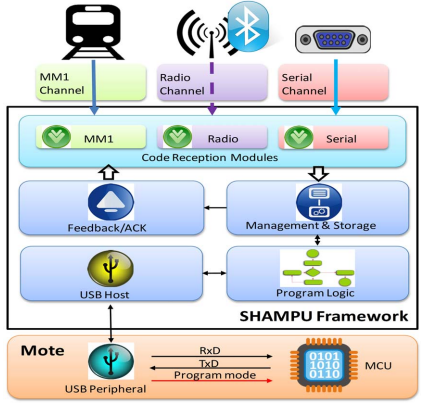
\includegraphics[scale=.5]{./pics/SHAMPUframework.png}
\caption{Overview of the SHAMPU Framework}\label{fig:shampuframework}
\end{figure}
The SHAMPU framework (see Figure \ref{fig:shampuframework}) itself is split into multiple modules. The Code Reception Module allows the use of different protocols to connect to and communicate with other SHAMPU enabled devices. For wireless communication SHAMPU uses an ANTAP1MxIB RF Transceiver Module, which supports the ANT protocol. The USB Host module is used to connect to the sensor node, which SHAMPU is attached to.

\section{ANT}
ANT \cite{DynastreamInnovationsInc.2013} is a wireless protocol which operates in the 2.4 GHz ISM Band. Originally developed in 2003 by Dynastream Innovations Inc. for the use wireless sensors. The ANT protocol is designed for the use in low power WSNs and puts a focus on scalability and ease of use.
\begin{figure}[h]
\centering
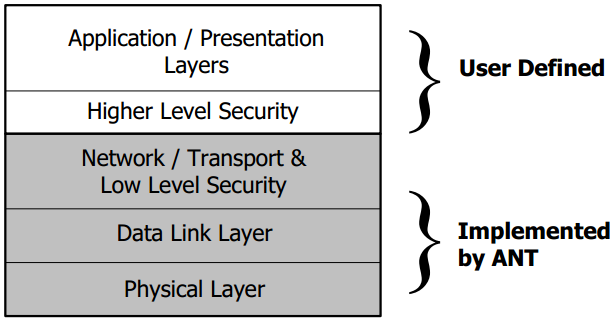
\includegraphics[scale=.5]{./pics/ANTstack.png}
\caption{OSI-Layer vs. ANT Protocol}\label{fig:osilayer}
\end{figure}
One of the advantages ANT has over other protocols, like Bluetooth or ZigBee is the high level of abstraction the ANT Protocol provides. This is achieved by the incorporation the first 4 OSI-layer (see Figure \ref{fig:osilayer}) into the ANT protocol and thus allowing even low-cost MCU to setup and maintain complex wireless networks.

\subsection{ANT Topology}

In order for ANT-Nodes to communicate with each other, they have to be part of a network. This is done be creating a channel and connection two or more different ANT nodes together. 
\begin{figure}[h]
	\centering
	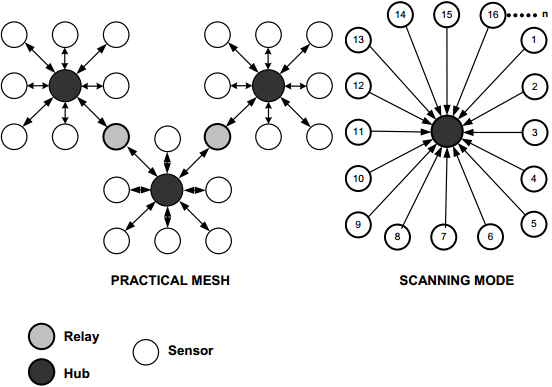
\includegraphics[scale=0.7]{./pics/ANTtopo.png}
	\caption{Example ANT Topologies}\label{fig:anttopo}
\end{figure}\\
\textbf{TODO}
\begin{itemize}
	\item{Explains what ANT nodes are}
	\item{Explain what channels are (for now in section ANT Channels)}
\end{itemize}

\subsection{ANT Channels}
Most of the available channel types are bidirectional, but the ANT protocol still differentiates between master and slaves nodes. While a master nodes mostly sends data and a slave nodes mostly receives data, the slave still has the ability to response to the incoming data.

The ANT protocol knows 125 different channels, each 1 MHz wide. Each Channel supports a data rate of 1 Mbps and up to 65533 nodes. To avoid interference between the channels isochronous selfadjusting TDMA technology is used, this allows the ANT nodes to change the transmit timings and even the frequency that is being used for the current channel.

\textit{Picture Process to establish a channel between master and slave nodes.}

The ANT protocol distinguishes between 2 different Channel types:
\begin{description}
\item{\textbf{Independent Channels}} \hfill \\ Independent Channels are used if there is only one ANT node, which is transmitting data. This allows 1:1 transmission, but also broadcasts.
\item{\textbf{Shared Channels}} \hfill \\ Shared Channels are used if a single ANT node needs to receive data from many nodes. This type of channel is made possible by the use of Shared Channel Address, however this reduces the amount of data that can be transmitted at a time.
\end{description}

\subsection{ANT Communication}
\textbf{TODO}
\begin{itemize}
	\item{Explain how each msg is structured}
	\item{Explain extended msg }
\end{itemize}

\section{ANTAP1MxIB RF}
In order to use the ANT protocol each SHAMPU-mote is equipped with an ANTAP1MxIB RF Transceiver Module. The module was chosen because of it's small form factor (20mm x 20mm) and very low power draw. The ANTAP1M can handle up to 4 ANT channels and a 1Mbps RF data rate, which is enough to setup and use the desired network topology.

\textbf{TODO}
\begin{itemize}
	\item{Explain how the Chip communicates with the SHAMPU node}
	\item{Explain how the Chip communicates with the host PC}
\end{itemize}

\chapter{Evaluation of SHAMPU}
In order to assess the capabilities of SHAMPU we plan and run experiments designed to evaluate the SHAMPU framework in the following three categories:
\begin{itemize}
	\item{\textbf{Communication Range}} 
	\item{\textbf{Communication Delay}} 
	\item{\textbf{Data Throughput}} 
\end{itemize}

For this we designed different scenarios, which test one or more of the described categories. The following section describes the experiments according to the following template:

\begin{description}
\item{\textbf{Name}} \hfill \\ The name of the experiment.
\item{\textbf{Description}} \hfill \\ A description of the experiment and the the category being evaluated.
\item{\textbf{Network Topology}} \hfill \\ A diagram of the network topology in which the experiment is run.
\item{\textbf{Result}} \hfill \\ The results of the experiment and any additional collected data.
\end{description}


\section{Experiment 1: Delay calculations between two nodes}

\section{Experiment 2: Delay calculations between multiple nodes}

\section{Experiment 3: Maximal communication Range}
\textit{Diagram for the experiment:  2 nodes   x meter apart.  with distances from 0.5 m to 30m  (floor in SM 3xx is 27m long)}
In this experiment we propose to test this theoretical limit, we set up two ANT radios next to each other. We then start moving the nodes away from each other until the connection breaks. We then start moving the nodes back together until a new connection is established.

\section{Experiment 4: Data Transfer between two nodes}
The ANT protocol promises a speed of up to 1 Mbps, 20 kbps of which are available for the application itself. In this experiment we try to determining the speed with which it is possible to move data to and form a SHAMPU device. We also try to determinate what effect the size of the payload and the number of the nodes in the network have on the transmission speed.

\section{Experiment 5: Reflash of a wireless sensor network}

\chapter{Conclusion}
\textbf{TODO}
\section{Summary}
\textbf{TODO}
\section{Future Work}
\textbf{TODO}

\bibliography{bibliography}
\end{document}